\section{Introduction}

\label{sec:Intro}

% Graph-- Uncertain Graph--Examples 
Graphs are widely used to capture the complex relationships in emerging applications, such as business to business (B2B) and social networks. 
Sometimes, the existence of the relationship between two entities is uncertain. For instance, in social networks, nodes represents individual users, while edges represent friendship or trust link among them.  Usually, the link is derived by inference and prediction models built on interaction details~\cite{Lin_B2B,Adar_Managing_2007,Kempe_Maximizing_2003}. And, edge probability denotes the accuracy of a link prediction, or the trust of one person on another. 
In these applications, the data can be modeled and shared as uncertain graphs whose edges carries a probability of existence. The probability represents the confidence that the relationship holds in reality. 

\begin{figure}[!htb]
  \vspace{-7pt}
    \subfigure[Social Trust Network]{\label{fig:socialNetwork}
      \begin{minipage}[l]{0.46\columnwidth}
        \centering
        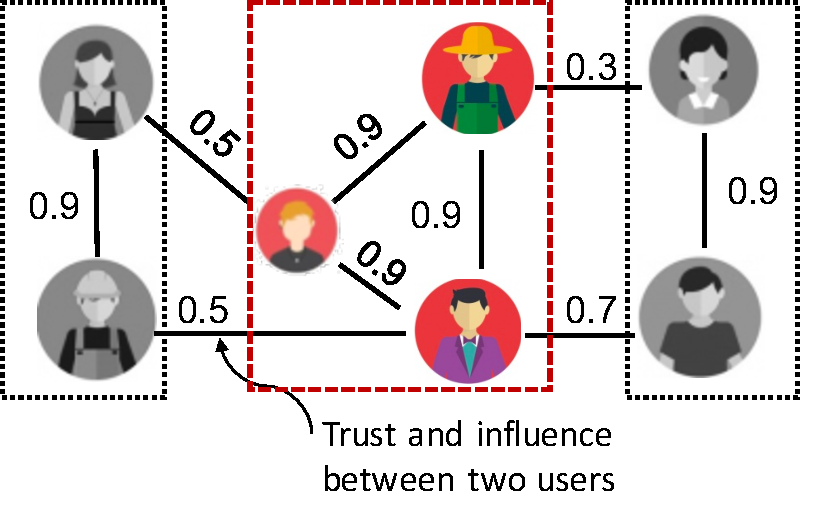
\includegraphics[height=2.7cm]{ill/SocialNetwork.pdf}
      \end{minipage}
      }
    \subfigure[B2B Network]{\label{fig:b2bNetwork}
      \begin{minipage}[l]{0.46\columnwidth}
        \centering
        \includegraphics[height=2.7cm]{ill/B2BNetwork.pdf}
      \end{minipage}
      }
    \vspace{-7pt}
    \caption{Real-world uncertain graphs with privacy concerns.}
    \label{fig:motivation}
    \vspace{-7pt}
\end{figure} 

% Sharing--Privacy--Examples 
These uncertain graphs are invaluable for scientific research and commercial applications~\cite{Kempe_Maximizing_2003,Cho_Friendship_2011}. However, sharing these uncertain graphs would violate the privacy of users or entities profiled inside. In social trust network, the trust relationships among users--- which greatly impact users' behaviors, are usually probabilistic.  They are useful in social interaction study and micro-targeting. While users are unwilling to share such confidential information with potential adversaries like Cambridge Analytica. In B2B networks, business operators also hesitate to share transaction patterns as it relates to  confidential business models. Such tension is raising the question of sharing uncertain graphs without compromising privacy. 


% State-of-Art 
A number of privacy preserving graph sharing schemes have been studied in the deterministic scenario~\cite{Liu_Towards_2008,Ying_Randomizing_2008,Wang2011,Liu_Privacy_2009,Nguyen_Anonymizing_2015,Sala_Sharing_2011,Xiao_Differentially_2014,lee2011}, though many problems still remain unexplored in the uncertain scenario.

\begin{figure}[!htb]
  \centering
  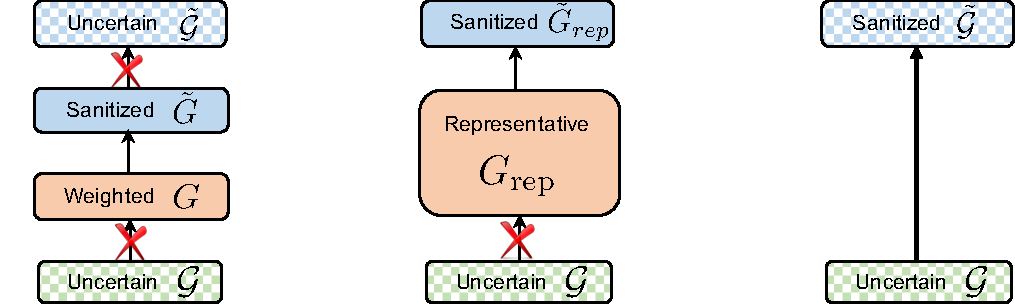
\includegraphics[width=0.9\linewidth]{ill/methods.pdf}
  \caption{XXXX.}
  \vspace{-14pt}
\end{figure}
%weight casting fails 
An obvious approach is to convert uncertain graph sharing problem into the deterministic case by casting edge probabilities as edge weights. 
Note that, one of the most important goals of sharing uncertain graphs is to maintain the data utility. 
However, by disregarding the possible world semantics of the uncertain graph, casting-based approach, as later illustrated, fails to reflect uncertain graph properties such as connectivity, dense subgraphs correctly~\cite{Zhao_Detecting_2014,Hua_Probabilistic_2010}. 
Hence, casting-based scheme could produce very poor result in the uncertain scenario even if the weighted graph anonymization algorithm is good. 

{\small Connectivity of deterministic subgraphs is generally measured by the concept of cut, which is defined as the sum of weights of intra edges. Generally, the bigger the cut, the harder to separate two subgraphs. In Figure~\ref{fig:motivation}(a), the equal cut $C(SG_{1},SG_{2})=C(SG_{3},SG_{2})=1$ implies the identical connectivity of $SG_{1}$ and $SG_{3}$ w.r.t $SG_{2}$. However, with the possible world semantics, we know the probability to separate $SG_{1}$ and $SG_{2}$ is $(1-0.5)^{2}=0.25$, and that to separate $SG_{2}$ and $SG_{3}$ is $(1-0.3)(1-0.7)=0.21$. Hence, in fact, $SG_{2}$ is closer to $SG_{1}$ than to $SG_{3}$.} 

Another approach proposed in our previous work~\cite{Xiao:2018}, called rep-based anonymization, is based on the idea of processing uncertain graph through representative instances~\cite{Parchas_Gullo_Papadias_Bonchi_2014}.
It first extracts a single deterministic representative instance $G$ that capture structural properties of the uncertain graph.
After that, anonymization can be then be proceed efficiently on $G$ using conventional algorithms, regardless of the uncertainty.  
However, Rep-An is is not always feasible. 
The detachment of edge uncertainty deteriorates the data utility. 

Conventional graph anonymization schemes are inadequate to share uncertain graphs with a desirable trade-off between privacy and utility. 
It is worthwhile to consider developing the specially optimized solution for handling following challenges. 

$\bullet$~\textup{\emph{Stochastic Privacy Attacks.}}~~Edge uncertainty plays an indispensable role in the uncertain graph model. It is impractical to discard them in the release.  
While the extra release of edge uncertainty makes privacy protection far more difficult as it empowers the adversary and makes the profiled entity more vulnerable. 
% To this end, we show the potential re-identification attack and present the corresponding solution. 

$\bullet$~\textup{\emph{Stochastic Utility Loss Metric.}}~~It is challenging to maintain the structure when the uncertain graph is modified to pursue anonymity. 
The structural distortion incurred is evaluated by the specially designed utility loss metric.  
It plays the key role in utility preserving. 
Unfortunately, existing graph utility loss metrics such as graph edit distance~\cite{Liu_Towards_2008}, spectrum discrepancy~\cite{Ying_Randomizing_2008}, community reconstruction error~\cite{Wang2011} and shortest path discrepancy~\cite{Liu_Privacy_2009} are not suitable in the uncertain scenario because of the ignorance of edge uncertainty.
% In this context, the discrepancy w.r.t standard uncertain graph reliability becomes a good criterion. It evaluates the connectivity difference in the context of the entire graph and meanwhile utilizes the possible world model. 

$\bullet$~\textup{\emph{Intractable Search Space.}}~~The goal is to find a sanitized graph with the desired level of privacy by as few graph mutations as possible. 
Even the simple deterministic graph anonymization problem, {\ie}, only with edge additions and deletions, is a NP-hard problem~\cite{Hartung_Theory_2015}. 
In the uncertain scenario, the edge modification is no longer a binary operation (addition/deletion), but can be infinite probability values. Exhaustive search is computationally intractable if the number of edges is large. 
This makes the problem of uncertain graph anonymization very challenging. 
 % Thus, we approximate the problem of interest via a randomized algorithm, which built on the basis of meta-heuristics. It excels in identifying a population of sanitized results with good quality.

In this work, we propose a solution tailored towards uncertain graphs via incorporating possible world semantics.  
It preserves as much the stochastic nature of the original uncertain graph as possible, while injecting enough structural noise to guarantee a chosen level of privacy.
Specifically, we make the following contributions.
\vspace{-5pt}
\begin{itemize}
\item We are the first to formulate the uncertain graph anonymization problem. 
 We show the potential re-identification attack and present the corresponding privacy notion. 
\item We propose an utility loss metric on the basis of reliability. It evaluates the connectivity difference in the context of the entire graph and also utilizes the possible world model. 
\item We propose a randomized algorithm with the hybrid of uncertainty-aware heuristics. It excels in identifying a population of sanitized results with good quality efficiently.
\item We conduct extensive experimental studies to demonstrate efficiency and practical utility of our algorithms.
\end{itemize}

The rest of the paper is organized as follows. In Section 2, we summarize related works and clarify our distinct privacy goal. In Section 3 we formulate the uncertain graph-anonymization problem. Sections 4 – 5 consider the anonymization problem in the context of uncertain graphs.  In Section 6 we apply our method to several real-world uncertain graphs, and demonstrate their efficiency and practical utility. 

